\documentclass[11pt,a4paper]{article}

% Paquetes básicos
\usepackage[utf8]{inputenc}
\usepackage[spanish,es-tabla]{babel}
\usepackage{amsmath, amssymb, amsfonts}
\usepackage{geometry}
\geometry{top=2.5cm, bottom=2.5cm, left=2.5cm, right=2.5cm}

% Manejo de imágenes y PDFs
\usepackage{graphicx}
\usepackage{float}
\usepackage{pdfpages}
\usepackage{adjustbox}

\begin{document}

% ---------------------------------------------------------
% CARÁTULA
% ---------------------------------------------------------
% Se incluye el PDF de la carátula compartida por el grupo
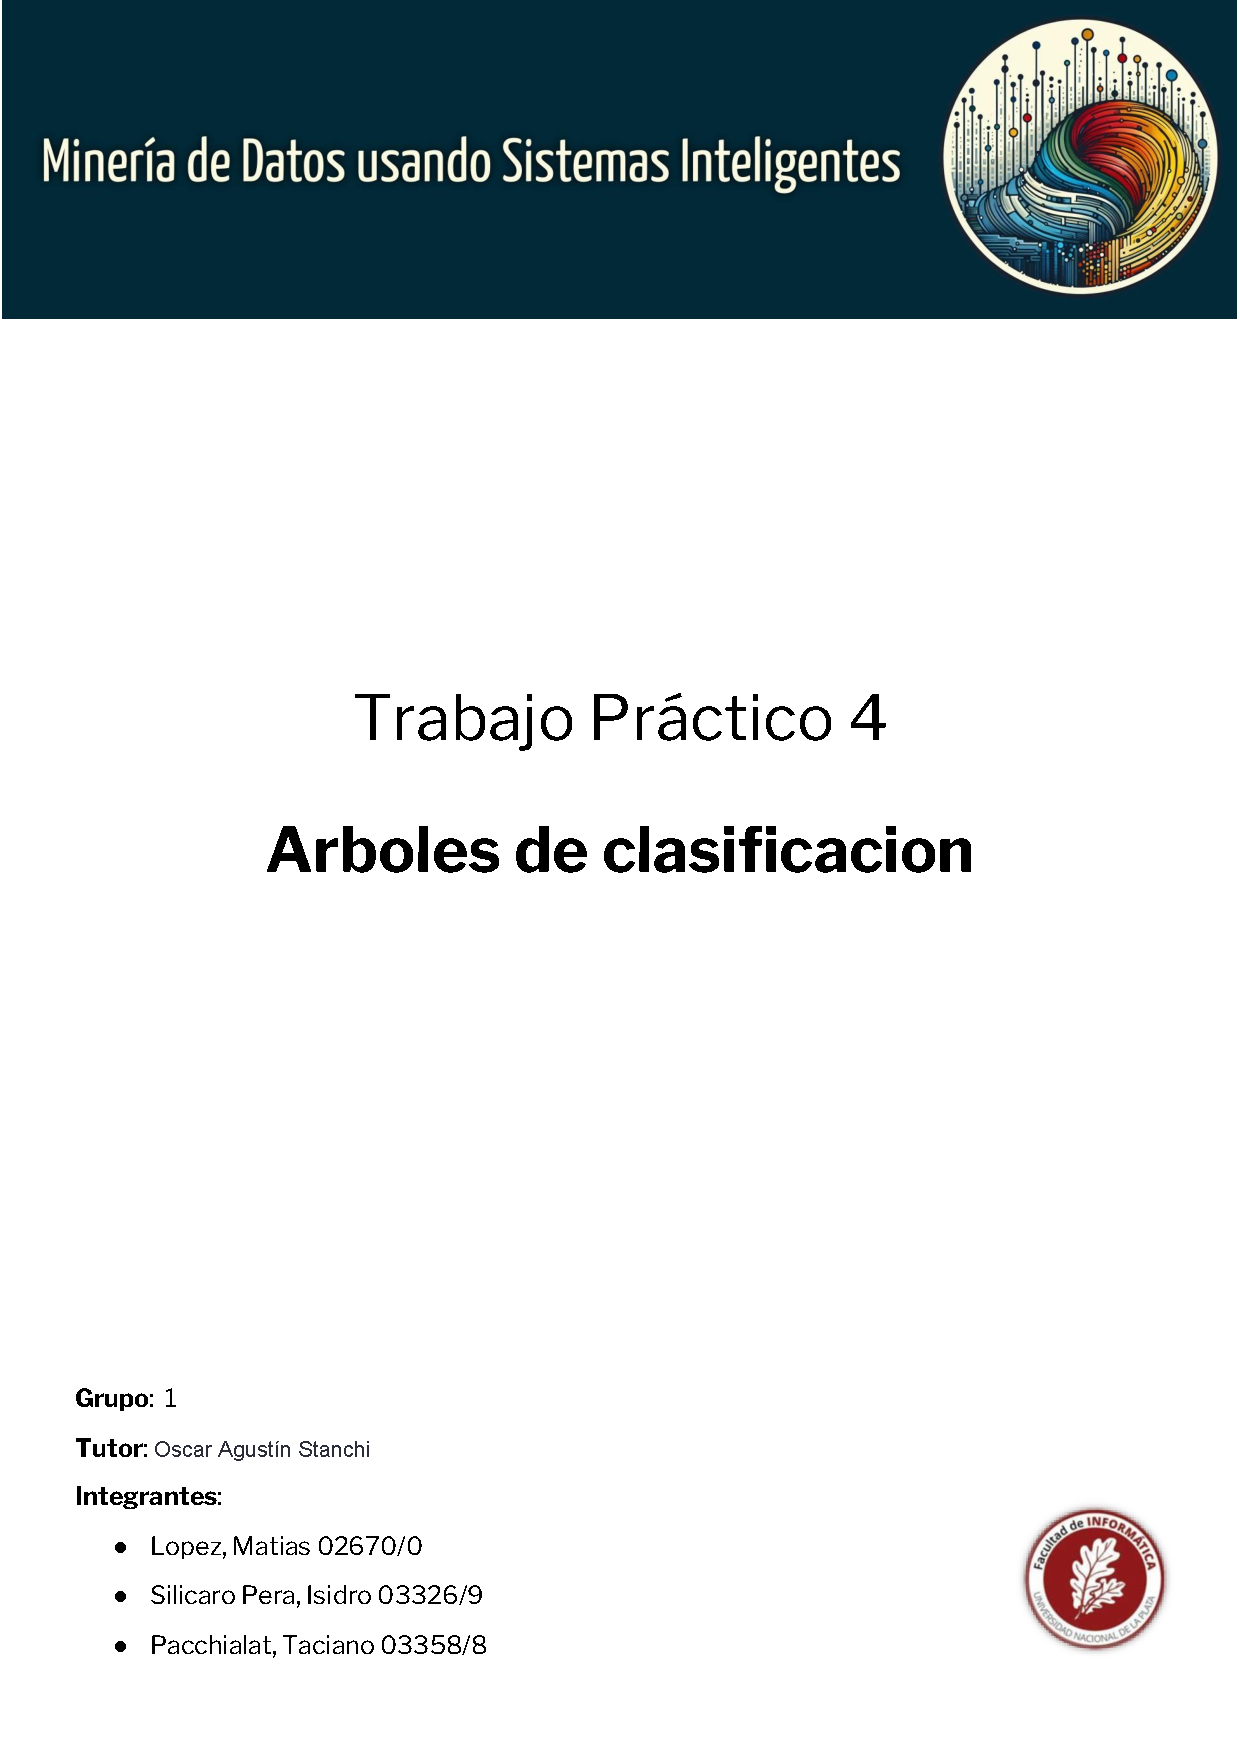
\includepdf[pages=-]{Caratula para entrega de TPs.pdf}

% ---------------------------------------------------------
% EJERCICIO 5: Construcción de árboles
% ---------------------------------------------------------
\section*{5. Construcción de árboles}

\subsection*{a) Construcción manual del árbol de clasificación C4.5}

A continuación se detalla la construcción manual de un árbol de clasificación C4.5 sin poda, utilizando la Ganancia de Información como criterio sobre los datos del archivo \textbf{trabajos\_ej4\_train.csv}. El objetivo es predecir si una persona obtendrá o no el trabajo según sus antecedentes.

A continuación se presentan los datos del conjunto de entrenamiento utilizados:

\begin{table}[H]
\centering
\begin{adjustbox}{width=0.9\textwidth}
\begin{tabular}{|c|c|c|c|c|c|}
\hline
\textbf{Instancia} & \textbf{Título universitario} & \textbf{Experiencia en el cargo} & \textbf{Cantidad de Trabajos Anteriores} & \textbf{Trabaja actualmente} & \textbf{Obtiene trabajo} \\ \hline
0 & SI & BAJA & 6 & SI & SI \\ \hline
1 & NO & BAJA & 6 & NO & NO \\ \hline
2 & NO & ALTA & 6 & NO & NO \\ \hline
3 & NO & ALTA & 6 & NO & NO \\ \hline
4 & NO & MEDIA & 6 & SI & NO \\ \hline
5 & SI & BAJA & 6 & NO & SI \\ \hline
6 & NO & BAJA & 6 & SI & NO \\ \hline
7 & NO & ALTA & 8 & SI & SI \\ \hline
8 & SI & ALTA & 8 & NO & SI \\ \hline
9 & NO & MEDIA & 8 & SI & NO \\ \hline
10 & NO & BAJA & 6 & NO & NO \\ \hline
11 & NO & MEDIA & 6 & NO & NO \\ \hline
12 & NO & MEDIA & 6 & NO & NO \\ \hline
13 & SI & ALTA & 9 & SI & SI \\ \hline
14 & NO & MEDIA & 9 & SI & SI \\ \hline
15 & NO & MEDIA & 9 & NO & SI \\ \hline
\end{tabular}
\end{adjustbox}
\caption{Conjunto de datos de entrenamiento para la construcción del árbol.}
\end{table}

En cada paso se presentan los valores de Entropía y Ganancia de Información para cada atributo evaluado.

Los desarrollos manuscritos de los cálculos y las divisiones sucesivas pueden consultarse de forma detallada en el \textbf{Anexo: Procedimientos Manuscritos} al final de este documento. La verificación de estos resultados se realizó contrastándolos con los scripts de Python provistos teóricamente.

\subsection*{c) Accuracy del árbol en el conjunto de entrenamiento}

El accuracy obtenido tras evaluar el árbol construido sobre el propio conjunto de entrenamiento es:

\[
\text{Accuracy}_{\text{train}} = \text{Valor}
\]

\newpage
% ---------------------------------------------------------
% EJERCICIO 7: Efecto del tamaño del árbol
% ---------------------------------------------------------
\section*{7. Efecto del tamaño del árbol}

En esta sección se analiza cómo la variación de los hiperparámetros impacta en el tamaño del árbol y en su rendimiento tanto en el conjunto de entrenamiento como de testeo. Se utilizó el archivo \textbf{diabetes\_nominal\_train} para el entrenamiento y \textbf{diabetes\_nominal\_test.xlsx} para la evaluación, empleando \textit{information gain} como medida de desorden y \textit{min\_error\_decrease} $= 0.01$.

\subsection*{a) Árbol con min\_samples\_split = 40 y min\_samples\_leaf = 20}

% Completar con la observación de la tasa de aciertos y el tamaño del árbol.

\subsection*{b) Árbol con min\_samples\_split = 100 y min\_samples\_leaf = 50}

% Completar con la observación del tamaño del árbol y el rendimiento.

\subsection*{c) Árbol con min\_samples\_split = 20 y min\_samples\_leaf = 10}

% Completar con la observación del tamaño del árbol y el rendimiento.

\subsection*{d) Análisis y Conclusiones}

\textbf{¿Qué ocurre con el tamaño y complejidad del árbol en cada caso?}
% Respuesta

\textbf{¿Se observan diferencias en la performance del árbol en ambos conjuntos de datos? ¿A qué se deben estas diferencias?}
% Respuesta

\vspace{0.5cm}

A modo de resumen, se presenta la siguiente tabla con los resultados de cada inciso:

\begin{table}[H]
\centering
\begin{tabular}{|l|c|c|c|}
\hline
\textbf{Inciso} & \textbf{c)} & \textbf{a)} & \textbf{b)} \\ \hline
\textit{min\_samples\_split} & 20 & 40 & 100 \\ \hline
\textit{min\_samples\_leaf}  & 10 & 20 & 50 \\ \hline
Tamaño del árbol             &    &    &    \\ \hline
\textit{Accuracy Train}      &    &    &    \\ \hline
\textit{Accuracy Test}       &    &    &    \\ \hline
\end{tabular}
\caption{Comparación del tamaño del árbol y accuracy para distintos hiperparámetros.}
\end{table}


% ---------------------------------------------------------
% ANEXO: PROCEDIMIENTOS MANUSCRITOS
% ---------------------------------------------------------
\newpage
\section*{Anexo: Procedimientos Manuscritos}

A continuación se adjuntan las capturas de los procedimientos y cálculos analíticos realizados manualmente para la resolución del Ejercicio 5.

\begin{figure}[H]
    \centering
    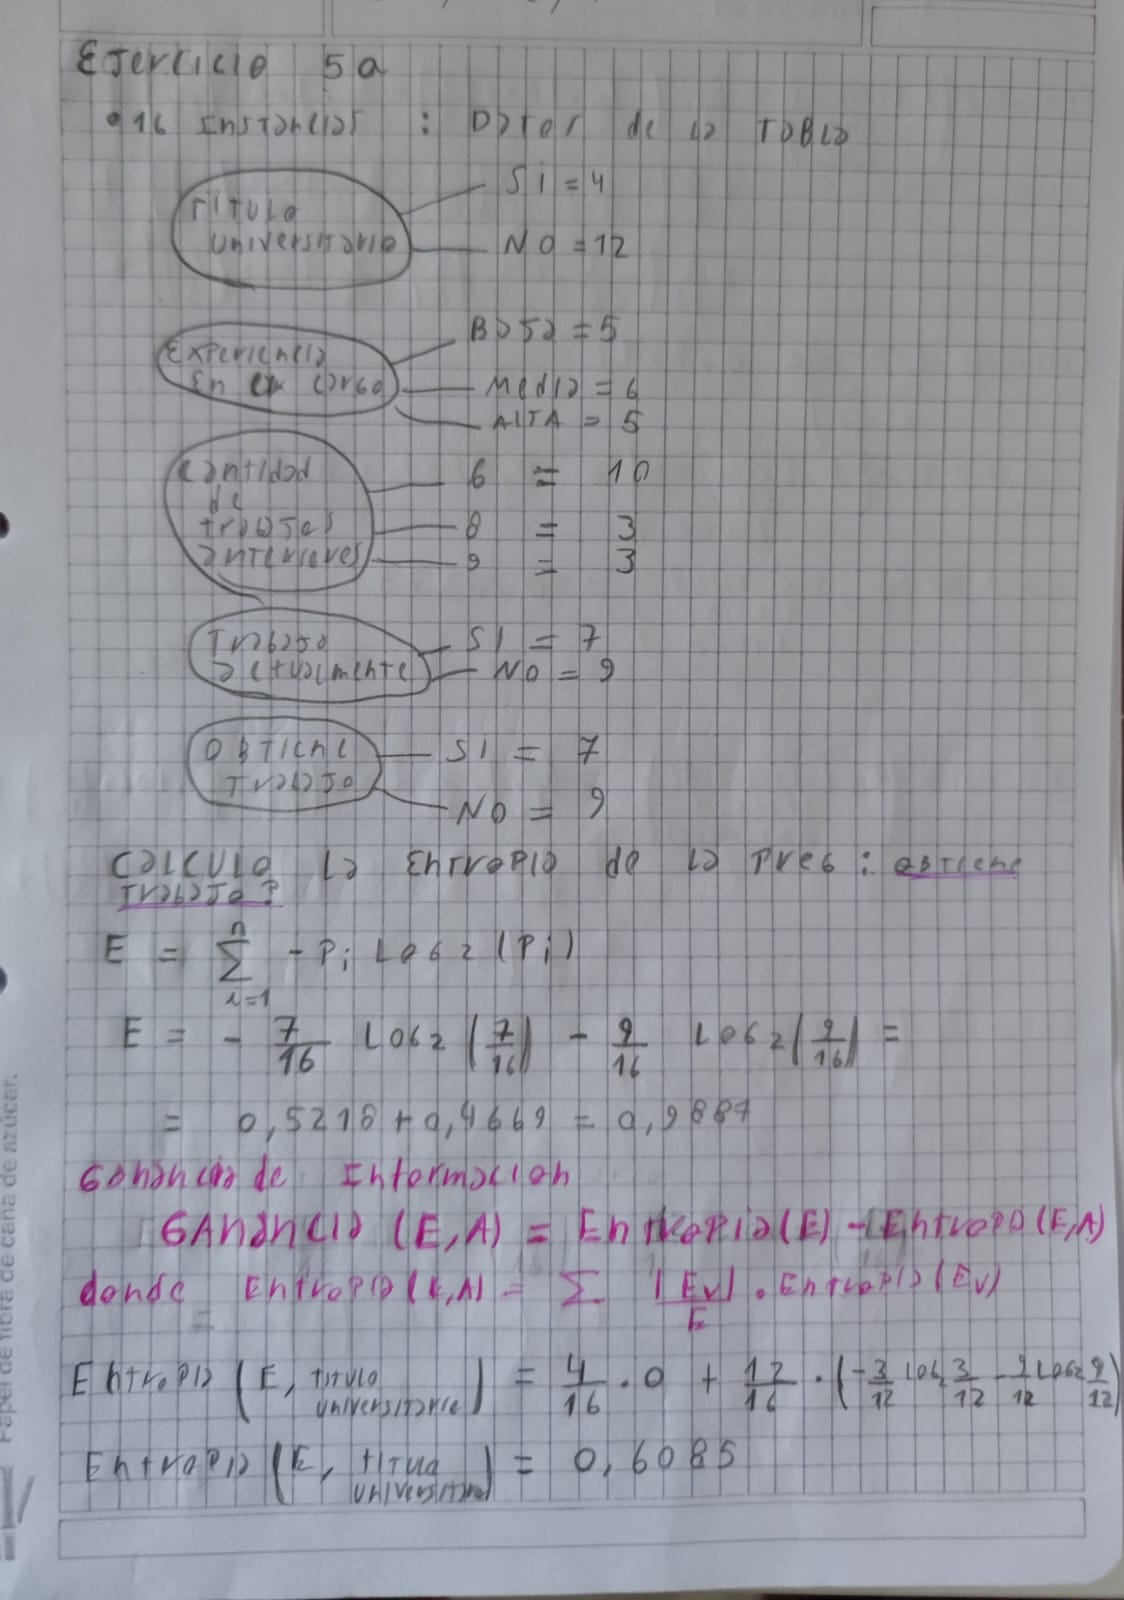
\includegraphics[width=0.9\textwidth]{Ejercicio5a-1.jpeg}
    \caption{Desarrollo manuscrito del Inciso A - Parte 1.}
\end{figure}

\begin{figure}[H]
    \centering
    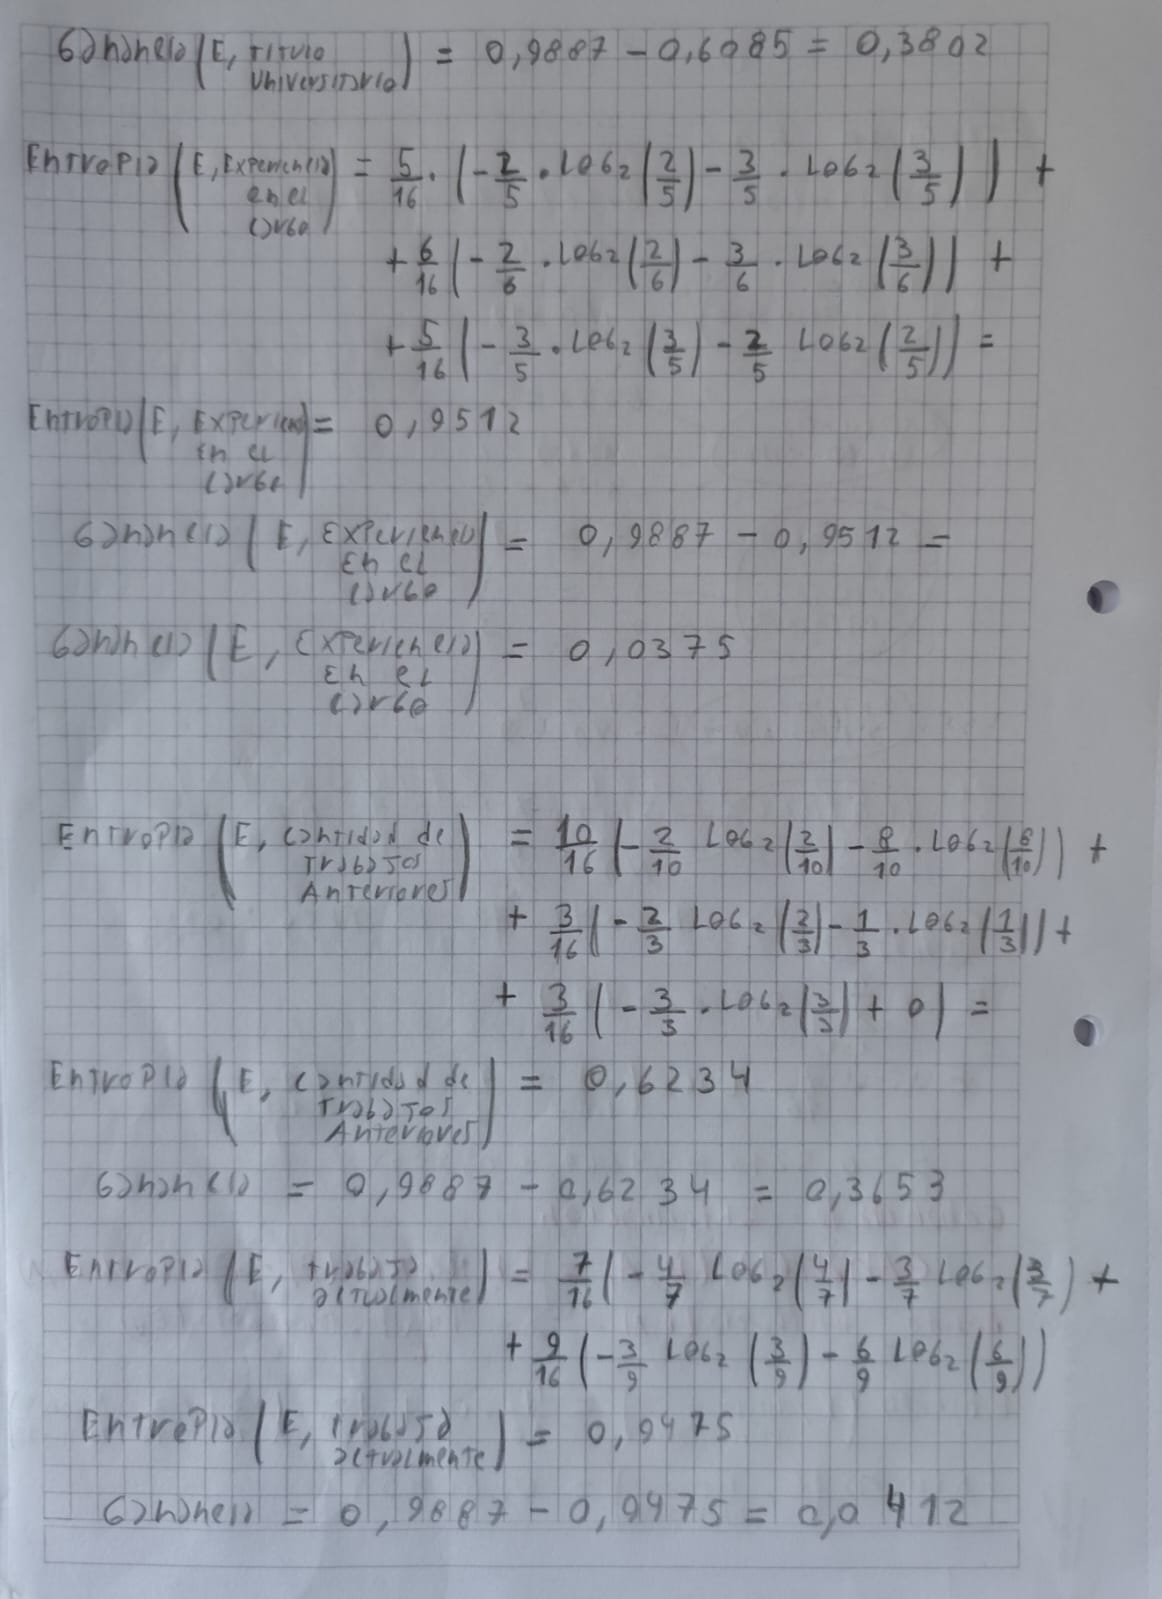
\includegraphics[width=0.9\textwidth]{Ejercicio5a-2.jpeg}
    \caption{Desarrollo manuscrito del Inciso A - Parte 2.}
\end{figure}

\begin{figure}[H]
    \centering
    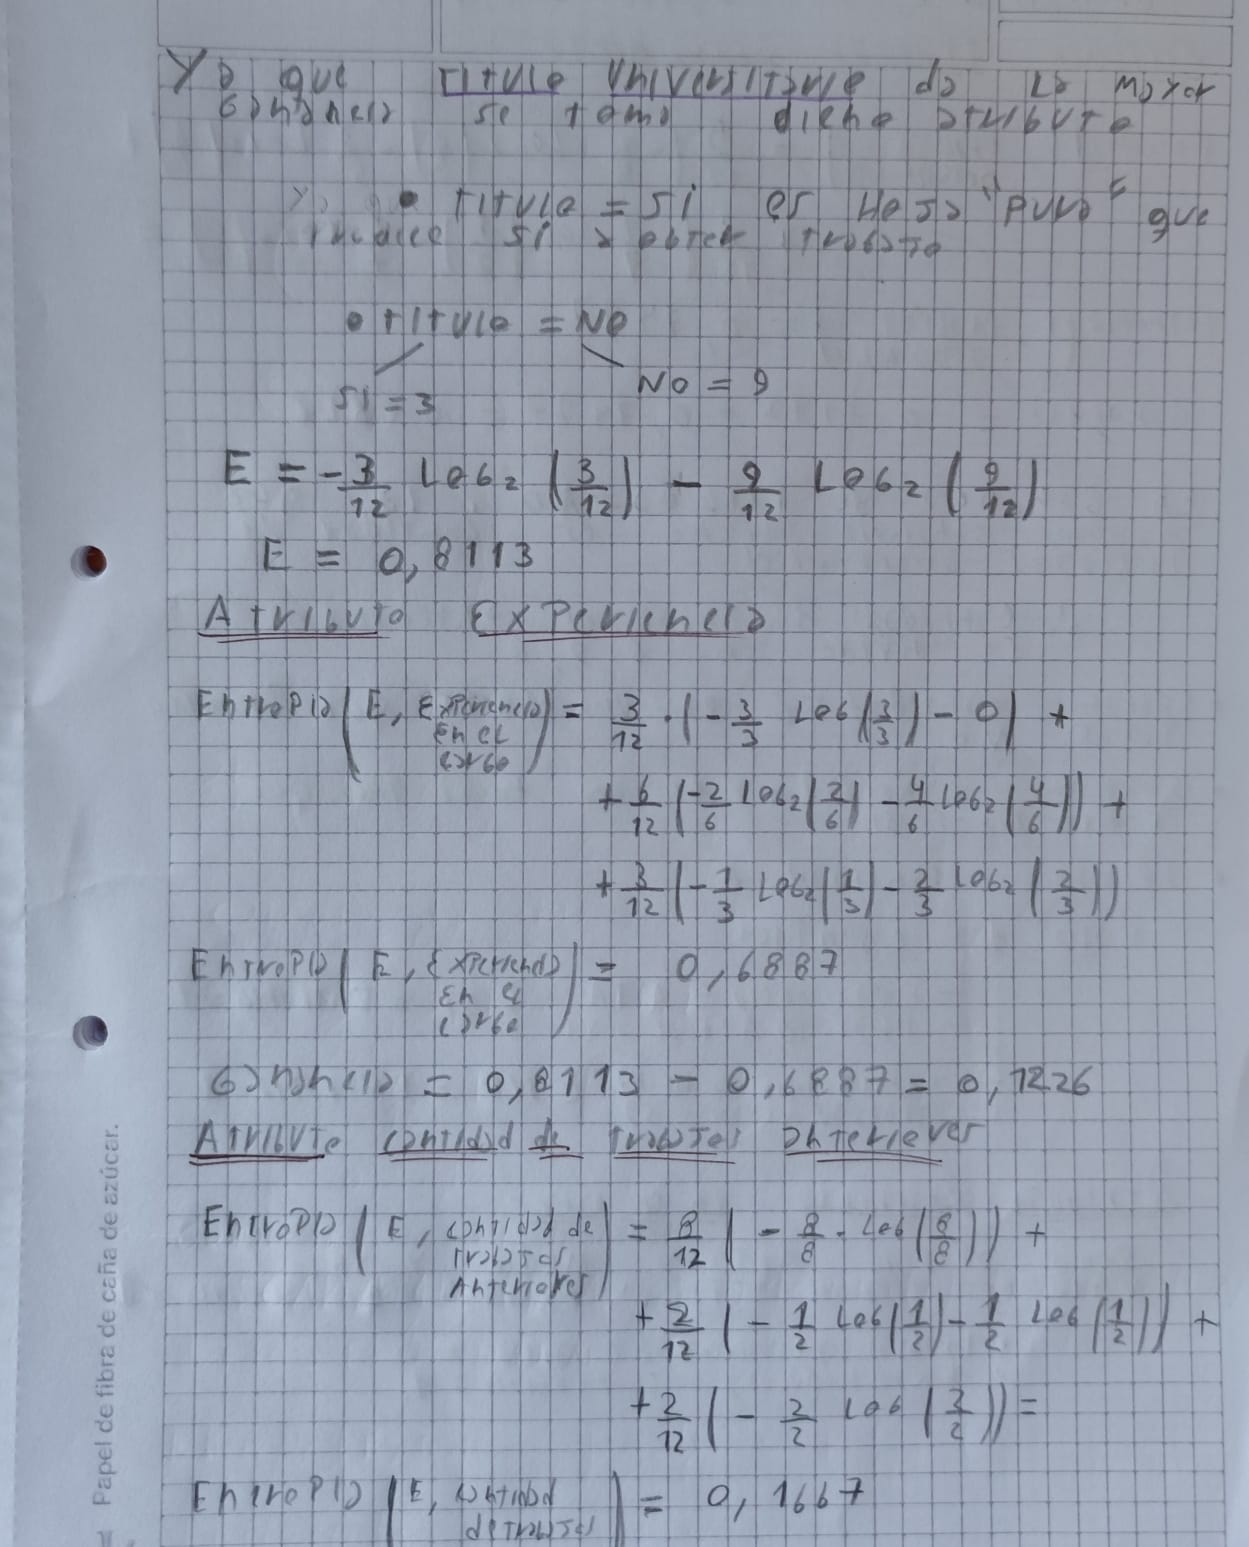
\includegraphics[width=0.9\textwidth]{Ejercicio5a-3.jpeg}
    \caption{Desarrollo manuscrito del Inciso A - Parte 3.}
\end{figure}

\begin{figure}[H]
    \centering
    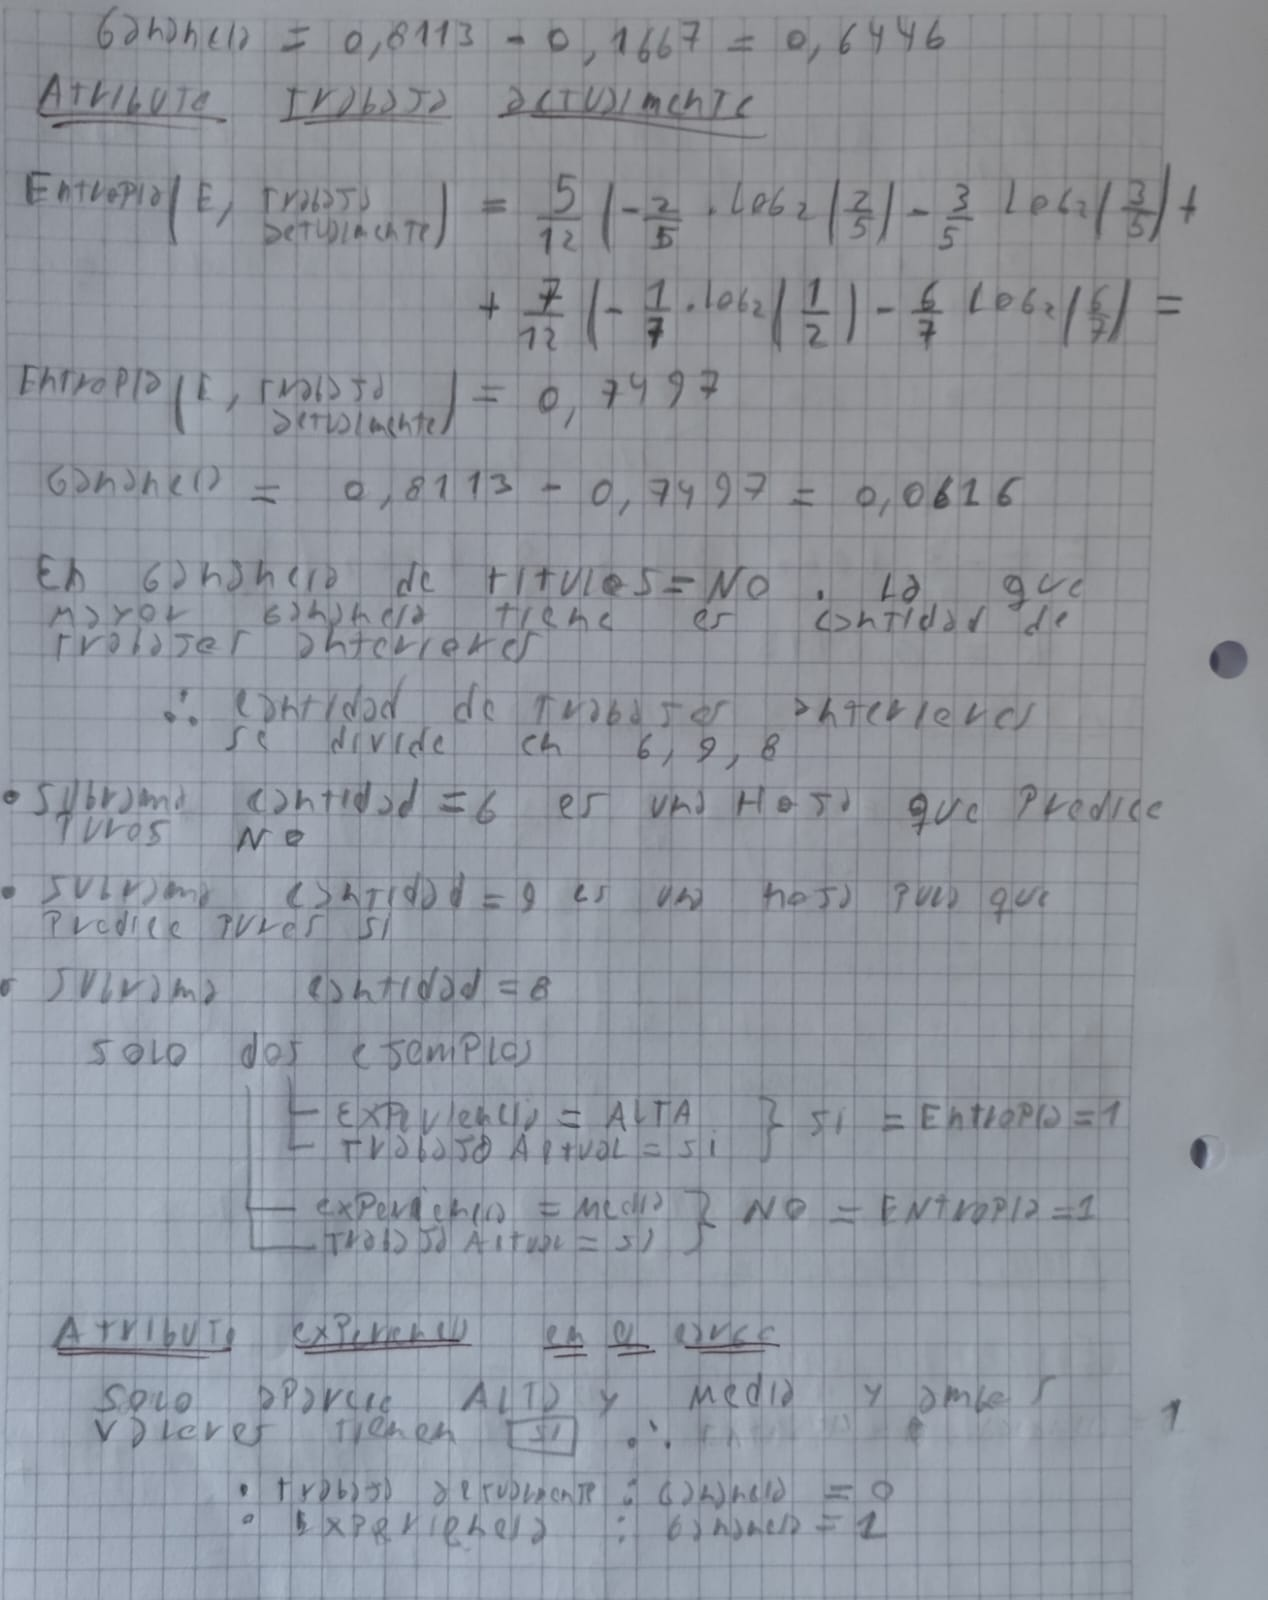
\includegraphics[width=0.9\textwidth]{Ejercicio5a-4.jpeg}
    \caption{Desarrollo manuscrito del Inciso A - Parte 4.}
\end{figure}

\begin{figure}[H]
    \centering
    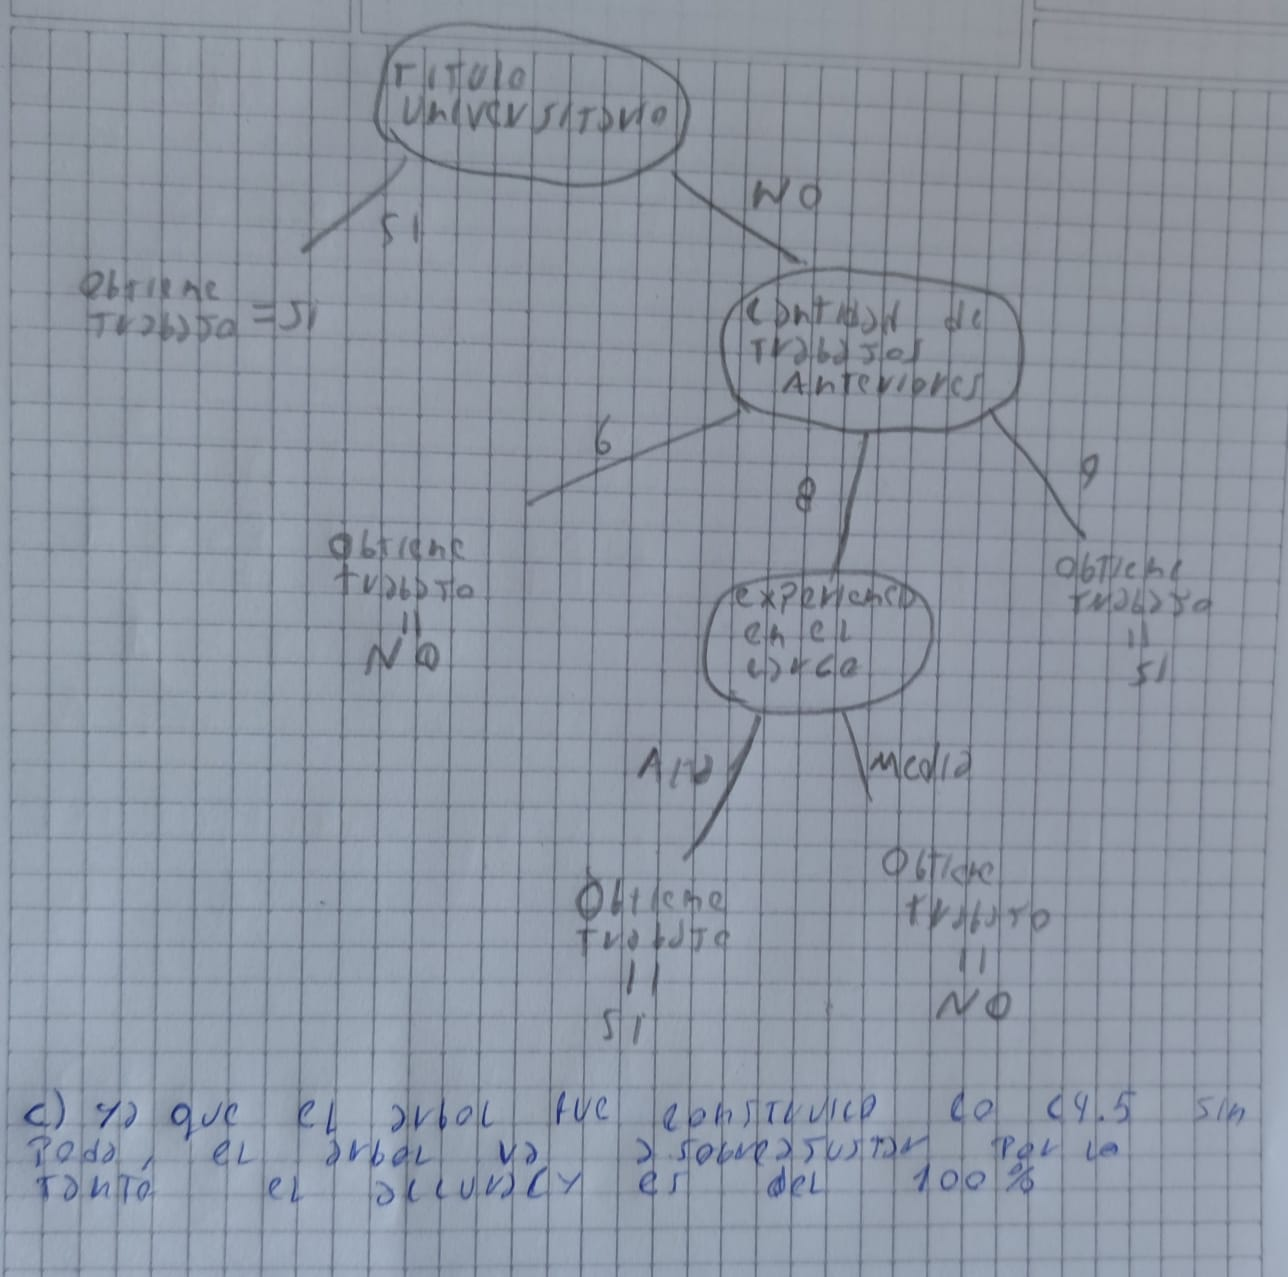
\includegraphics[width=0.9\textwidth]{Ejercicio5c.jpeg}
    \caption{Desarrollo manuscrito del Inciso C.}
\end{figure}

\end{document}